\documentclass[12pt]{article}

\usepackage{tabto}
\usepackage[english]{babel}
\usepackage[utf8]{inputenc}
\usepackage{amsmath}
\usepackage{graphicx}
\usepackage[colorinlistoftodos]{todonotes}
\usepackage{float}
\restylefloat{figure}
\usepackage{subfig}
\usepackage{amssymb}

\usepackage[top=1.0in,bottom=1in,right=.5in,left=.5in,headheight=50pt,headsep=0.5cm]{geometry}
\usepackage{siunitx}
\usepackage{mcode}
\usepackage{url}
\usepackage{verbatim}
\usepackage{tipa}
\usepackage{fancyhdr}
\usepackage{enumitem}
\usepackage{color}
\definecolor{dkgreen}{rgb}{0,0.6,0}
\definecolor{gray}{rgb}{0.5,0.5,0.5}
\definecolor{mauve}{rgb}{0.58,0,0.82}
\lstset{frame=tb,
	language=R,
	aboveskip=3mm,
	belowskip=3mm,
	showstringspaces=false,
	columns=flexible,
	numbers=none,
	keywordstyle=\color{blue},
	numberstyle=\tiny\color{gray},
	commentstyle=\color{dkgreen},
	stringstyle=\color{mauve},
	breaklines=true,
	breakatwhitespace=false,
	tabsize=3,
	frame=single
}
\newcommand{\squeezeup}{\vspace{-5mm}}

\pagestyle{fancy}
\fancyhf{}
\rhead{Bruce Goldfeder}
\lhead{CSI 758 Spring 2017 HW \#1}
\cfoot{Page \thepage}
\usepackage{sectsty}
\newcommand{\Rho}{\mathrm{P}}

\sectionfont{\fontsize{12}{15}\selectfont}

\subsectionfont{\fontsize{12}{15}\selectfont}

\title{CSI 758 Spring 2017 HW\#1}

\author{Bruce Goldfeder}

\date{\today}
\providecommand{\e}[1]{\ensuremath{\times 10^{#1}}}

\renewcommand{\thesubsection}{\thesection.\alph{subsection}}

\begin{document}
\maketitle
\NumTabs{12}

1.	Load the image bird.jpg. Create a new image in which the red channel data is placed in the green channel, the green channel information is placed in the blue channel, and the blue channel information is placed in the red channel. Show your code and paste your result.\\

The following code reads in the bird.jpg image, then performs a self transpose which creates three arrays of red, green, and blue.  I then build an empty zeros matrix of the same dimensions as the original and put each color band in the reordered sequence.  The code is shown below:
\begin{lstlisting}[language=Python]
# -*- coding: utf-8 -*-
"""
Created on Mon Feb 13 19:58:50 2017

@author: bruce
"""

import scipy.misc as sm
import numpy as np

# Question #1 channel switch - red to green, green to blue, blue to red
# read in the image bird.jpg
bdata = sm.imread("bird.jpg")
bdata.shape

x,y,rgb = bdata.shape

red,green,blue = bdata.T
sm.imsave('r.png', red )
sm.imsave('g.png', green )
sm.imsave('b.png', blue )

c = np.zeros( (y,x,rgb) ) 
c[:,:,0] = blue
c[:,:,1] = red
c[:,:,2] = green
 
ct = np.transpose(c,axes=(1,0,2))

sm.imsave("gbr.jpg",ct)
\end{lstlisting}
The images are shown below:\\

\begin{figure}[ht!]%
    \centering
    \subfloat[Original Image]{{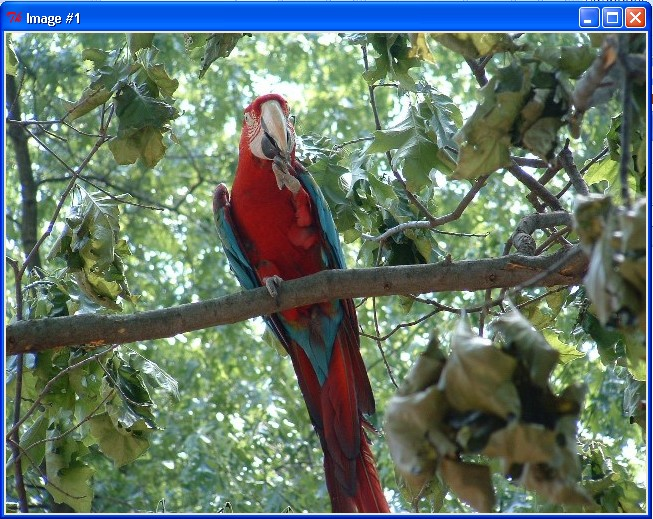
\includegraphics[width=5cm]{bird.jpg} }}%
    \qquad
    \subfloat[GBR Image]{{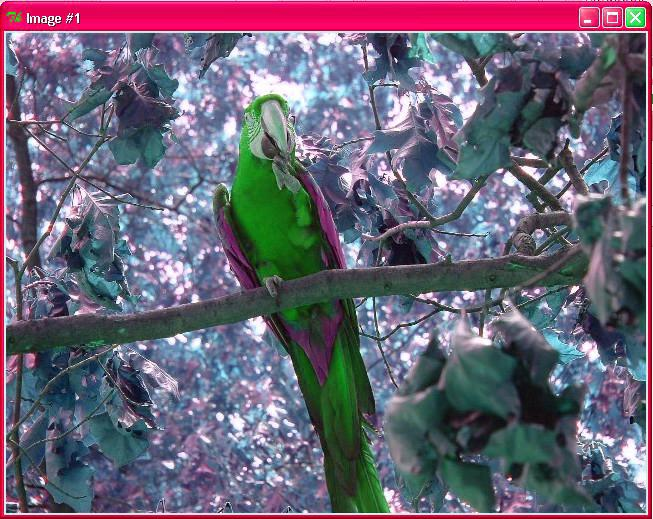
\includegraphics[width=5cm]{gbr.jpg} }}%
    \caption{Original and GBR images side by side}%
    \label{fig:example}%
\end{figure}

2.	Write the notation for the following situation. Load the bird image, replace the red channel with the square root of the red channel values, replace the blue channel with the square of the blue channel values, and keep the green channel unchanged.\\

Read in the file:\\
$ \boldsymbol{a}[\vec{x}]$ = bird.jpg\\\\
Use Channel Separation to access individual channels:\\
$
\begin{Bmatrix} 
\boldsymbol{R}[\vec{x}]\\ 
\boldsymbol{G}[\vec{x}] \\ 
\boldsymbol{B}[\vec{x}]  
\end{Bmatrix} = \boldsymbol{a}[\vec{x}]$  \\\\
Replace the red channel with the square root of the red channel values\\\\
$\boldsymbol{b}[\vec{x}] =
\begin{Bmatrix} 
\sqrt{\boldsymbol{R}[\vec{x}]}\\ 
\boldsymbol{G}[\vec{x}] \\ 
\sqrt{\boldsymbol{B}[\vec{x}]}  
\end{Bmatrix}$ \\ 

\vspace{5mm}

3.	Write a script to convert the bird image to gray scale, find the maximum value, and the location(s) of the maximum.\\
Code is below:
\begin{lstlisting}[language=Python]
# -*- coding: utf-8 -*-
"""
Created on Wed Feb 15 19:45:16 2017

@author: bruce
"""

import scipy.misc as sm
import numpy as np
from scipy.ndimage import label

# Question #1 channel switch - red to green, green to blue, blue to red
# read in the image bird.jpg
bdata = sm.imread("bird.jpg",flatten=True)
bdata.shape

intdata = bdata.astype(int)
theMax = intdata.max()

adata = (intdata == 255)
b,n = label(adata)
c,d = np.nonzero(b)

maxList = np.column_stack([c,d])
np.set_printoptions(threshold=np.inf)
print(maxList)
np.set_printoptions(threshold=None)
sm.imsave("whites.png",adata)
\end{lstlisting}
The maximum value came to 255 (after casting to int).
The array of max values is as follows:
\begin{verbatim}
[[ 40 326]
 [ 45 261]
 [ 46 260]
 [ 78 272]
 [ 80 273]
 [ 81 266]
 [ 85 259]
 [ 85 260]
 [ 87 283]
 [ 88 260]
 [ 88 268]
 [ 90 294]
 [ 90 297]
 [ 91 286]
 [ 91 444]
 [100 407]
 [110 396]
 [111 405]
 [116 401]
 [121 397]
 [143  33]
 [169 528]
 [227 554]
 [330 379]
 [339 170]
 [340 485]
 [355 594]
 [412 273]]
\end{verbatim}
Presented in image form here are where the 27, pixels with value of 255 are.
\begin{figure}[H]
\begin{flushleft}
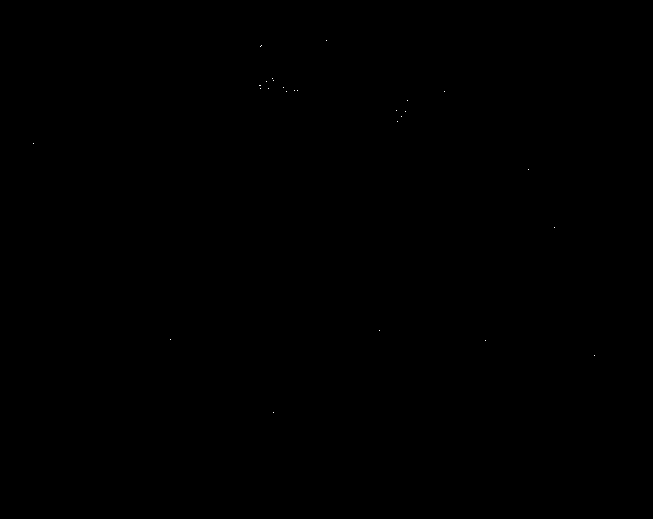
\includegraphics[scale=.8]{whites.png}
\end{flushleft}
\end{figure}

4.	Use the geos.png image. Use the ndimage.label function to isolate the objects. Then find the center of mass of the largest circle.\\
Code is below:
\begin{lstlisting}[language=Python]
# -*- coding: utf-8 -*-
"""
Created on Wed Feb 15 21:34:59 2017

@author: bruce
"""

import scipy.misc as sm
import numpy as np
import scipy.ndimage as nd

# Question #1 channel switch - red to green, green to blue, blue to red
# read in the image bird.jpg
bdata = sm.imread("geos.png")
bdata.shape

adata = (bdata < 255 )
b,n = nd.label( adata )
#c,d = np.nonzero(b)
#shapeList = np.column_stack([c,d])
c = (b == 4)
sm.imsave("bigC.png",c)

com = nd.center_of_mass(c)

print(com)
\end{lstlisting}

The label function provided isolation of the 5 shapes and selecting where the value was equal to 4 gave me the big circle.  The center of mass calculation came to (350.0, 300.0).  I saved these off as the images below:
\begin{figure}[ht!]%
    \centering
    \subfloat[Isolation using label]{{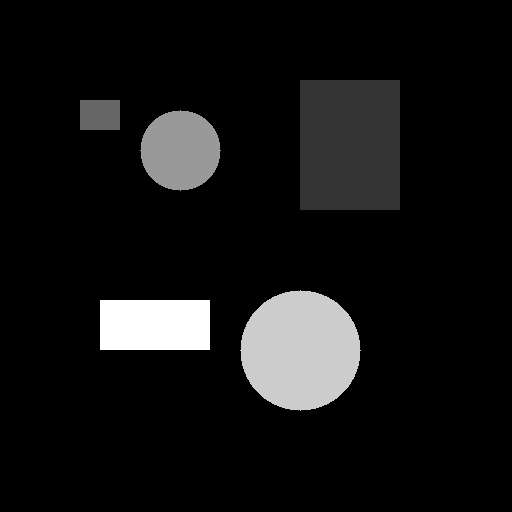
\includegraphics[width=5cm]{foo.png} }}%
    \qquad
    \subfloat[selected big circle]{{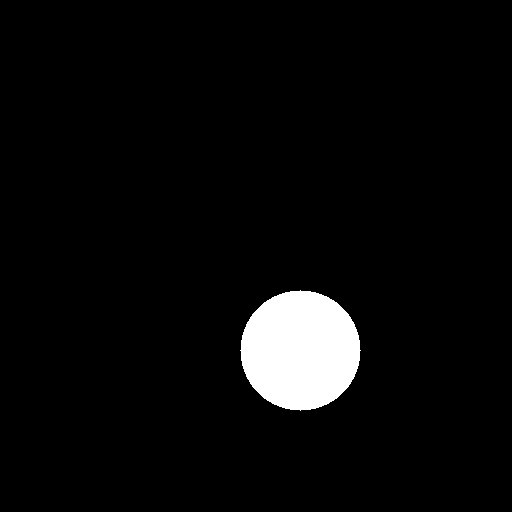
\includegraphics[width=5cm]{bigC.png} }}%
    \caption{Isolation and Selection}%
    \label{fig:example}%
\end{figure}

5.	Write the operator notation for the following actions:
\begin{enumerate}[label=(\alph*),leftmargin=2\parindent]
\item Start with a color image $ \boldsymbol{a}[\vec{x}]$. This has values ranging from 0 to 255. This size of the image frame is V×H.
\item	Convert to a gray scale image.
\item	Smooth this image with a smoothing factor of 2.
\item	Change all values less than 5 to 0. (noise removal)
\item	Find the center of mass.
\item	Move the image so that the center of mass is in the center of the frame.
\item	Rotate the image by 20 degrees.
\end{enumerate}
a. Read in the image as $ \boldsymbol{a}[\vec{x}]$ with dimensions V x H\\
b. Area A = V x H\\
c. Use Color Transformation where $n$, the model is L (gray scale) $ \boldsymbol{b}[\vec{x}] = \mathcal{L}_n\boldsymbol{a}[\vec{x}]$ this creates a gray scale image.\\
d. Smooth using a factor of 2, $ \boldsymbol{c}[\vec{x}] = 
S_2\boldsymbol{b}[\vec{x}]$ \\
e. Use a Threshold operator to remove values less than 5, $ \boldsymbol{d}[\vec{x}] = \Gamma_{<5}\boldsymbol{c}[\vec{x}]$ \\
f. Find the center of mass, $ [\vec{v}] = \boxtimes \boldsymbol{d}[\vec{x}]$, then use Plop to make this the new center,  $ \boldsymbol{e}[\vec{x}] = U_{[\vec{v}]}\boldsymbol{d}[\vec{x}]$ \\
g. Rotate the image by 20 degrees, $ \boldsymbol{f}[\vec{x}] = R_{20,[\vec{v}]}\boldsymbol{e}[\vec{x}]$ \\





6.	Load the bird image and call this image $ \boldsymbol{a}[\vec{x}]$ Create an image of a solid circle (use the Circle function) that is in a frame that is the same size as the original image. The circle should be located and sized such that it encompasses the whole bird head. (You may want to use anther program such as Gimp to determine the location and size of this circle.)  Smooth this circle so that the middle still has pixel values of 1 or very nearly 1 and the outer 10 (or so) pixels smoothly go from values of about 1 to about 0. Call this image b[x]. Create a new image from $ \boldsymbol{c}[\vec{x}]= \boldsymbol{a}[\vec{x}] \times \boldsymbol{b}[\vec{x}]$.\\\\
Using Gimp, I opened up the "pointer" dialog box to give me the x,y coords of where the pointer was at.  I found the smallest circle that would cover the parrot's head by finding the vertical top and vertical bottom of the face of the parrot.  These coordinates came to [270,90] to [270,160].  From this I used your mgcreate code to make the circle, then scipy.signal.cspline2d to smooth the edge.  Then I copied this 2D mask three times into a 3D matrix of zeros and multiplied this with the original image.  Now I have a cool parrot head with fuzzy edges! Fun!\\
\begin{lstlisting}[language=Python]
# -*- coding: utf-8 -*-
"""
Created on Wed Feb 15 22:30:07 2017

@author: bruce
"""

import scipy.misc as sm
import scipy.signal as sg
import numpy as np
import mgcreate as mg


# Question #1 channel switch - red to green, green to blue, blue to red
# read in the image bird.jpg
bdata = sm.imread("bird.jpg")
bdata.shape

mask = mg.Circle((519,653),(125,270),35)

b = sg.cspline2d(mask,1000)
sm.imsave("mask.png",b)

w, h = b.shape
mask3d = np.zeros((w, h, 3))
mask3d[:, :, 0] = b
mask3d[:, :, 1] = b
mask3d[:, :, 2] = b

sm.imsave("mask3d.png",mask3d)
     
maskParrot = bdata * mask3d
      
sm.imsave("maskParrot.png",maskParrot)
\end{lstlisting}
Here are the images of the original, the smoothed mask, and the final output
\begin{figure}[ht!]%
    \centering
    \subfloat[Original Image]{{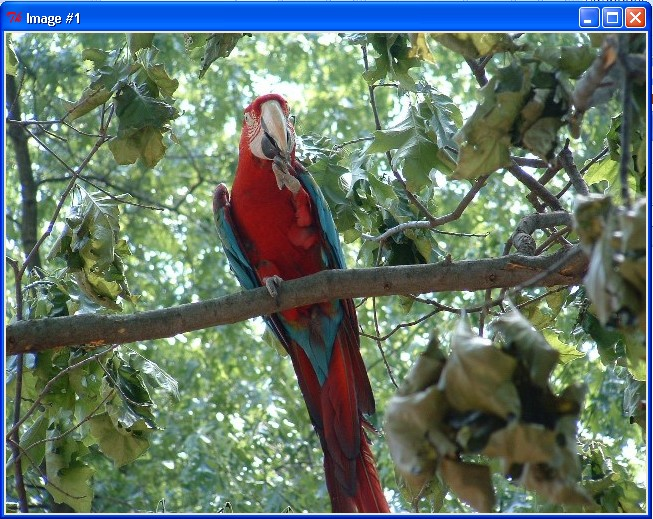
\includegraphics[width=5cm]{bird.jpg} }}%
    \qquad
    \subfloat[Mask with smoothing]{{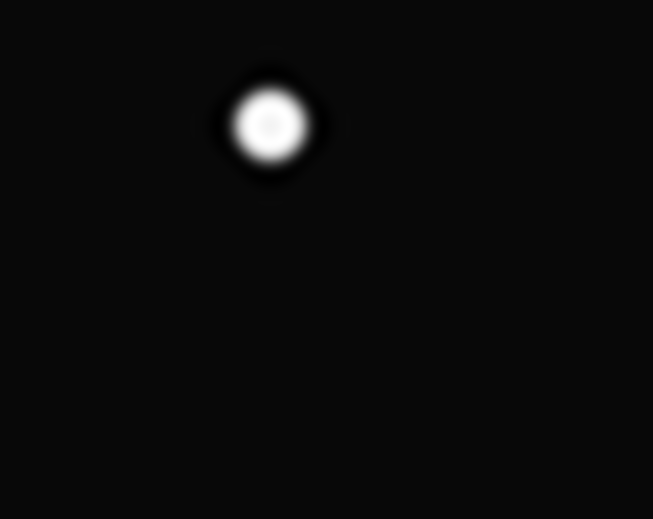
\includegraphics[width=5cm]{mask3d.png} }}%
    \qquad
    \subfloat[Multiplication of two images]{{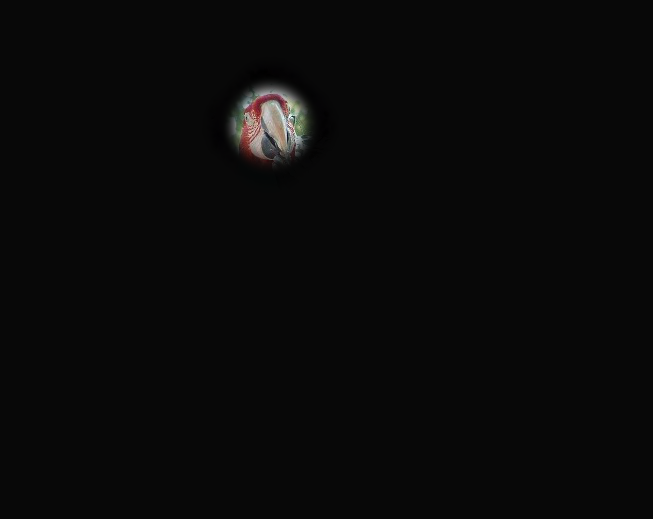
\includegraphics[width=5cm]{maskParrot.png} }}%
    \caption{Fuzzy Edged Parrot Head}%
    \label{fig:example}%
\end{figure}





\end{document}